\documentclass[11pt, letterpaper, includehead]{article}

%%%%%%%%%%%%%%%%%%%%% Pre-document %%%%%%%%%%%%%%%%%%%%%
\usepackage{fancyhdr}  % Allow for headers
\usepackage{graphicx}  % Allow for figures 
\usepackage{float}     % Allow for figure inserted in specified location
\usepackage{textcomp}  % Trade mark symbol
\usepackage{multicol}
\usepackage{amsmath}

\setlength{\parindent}{0pt} % Remove auto paragraph indents

% Get rid of those big ass margins
\usepackage[margin=1in]{geometry}

% Table cell formatting
\setlength{\arrayrulewidth}{0.25mm}
\setlength{\tabcolsep}{11pt}
\renewcommand{\arraystretch}{1.2}

\begin{document}

%%%%%%%%%%%%%%%%%%%%% Title Page %%%%%%%%%%%%%%%%%%%%%
\begin{titlepage}
  \begin{center}
    \Huge{\textbf{Lab 3}}\\
    \Huge{Vectors}
    \vfill
    \begin{figure}[H] % H makes the figure insert at the position in the document
      \centering 
      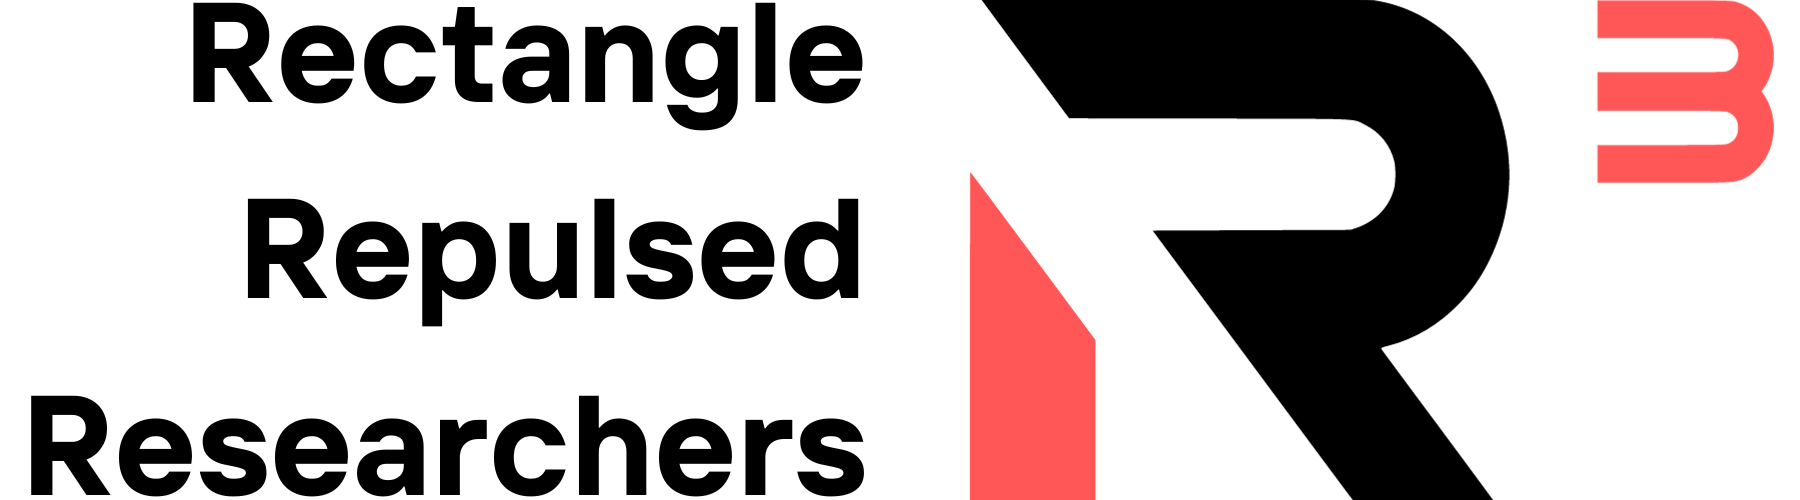
\includegraphics[width=6cm]{../logo.png}
    \end{figure}
    \large{\textbf{Rectangle Repulsed Researchers}}\\
    \large{Julian Barossi, Liam Gilligan, Stephanie L'Heureux}\\
    \vspace{0.5cm}
    \normalsize
    \today
  \end{center}
\end{titlepage}

%%%%%%%%%%%%%%%%%%%%% TABLE OF CONTENTS %%%%%%%%%%%%%%%%%%%%%
\tableofcontents
\pagebreak % Move to next page

% Add a nice fancy header
\pagestyle{fancy}
\fancyhead{}
\fancyhead[C]{\textbf{Lab 3:} Vectors}

\pagebreak 

%%%%%%%%%%%%%%%%%%%%% ADDING TWO VECTORS %%%%%%%%%%%%%%%%%%%%%
\section{Adding Two Vectors} % 1

%%%%%%%%%%%%%%%%%%%%% GIVEN VECTORS %%%%%%%%%%%%%%%%%%%%%
\subsection{Given vectors} % 1.1
The force vectors given were $35g$ at an angle of $60^{\circ}$ and $55g$ at an angle of $160^{\circ}$

\subsubsection{Find components} % 1.1.1
The $x$ and $y$ components of a vector are defined as a the amount the vector 
points along each axis. Vector components can be calculated using the Southern 
California Approach\textsuperscript{TM} or SOCA in which the component opposite to
$\theta$ is found by $\pm F \sin\theta$ and the adjacent to $\theta$ is $\pm F \cos\theta$

\begin{multicols}{2}
  \centering{\textbf{Force 1}}
  $$F_1 = mg$$
  $$F_1 = 35g \cdot \frac{1kg}{1000g} \cdot 9.80m/s^2$$
  $$F_1 = 0.343N$$

  $$F_{1_x} = F_1\cos\theta$$
  $$F_{1_x} = 0.343N\cos60^{\circ}$$
  $$F_{1_x} = 0.1715N \Rightarrow 0.172N$$
  $$\boxed{F_{1_x} = 0.172N}$$

  $$F_{1_y} = F_1\sin\theta$$
  $$F_{1_y} = 0.343N\sin60^{\circ}$$
  $$F_{1_y} = 0.2970467...N \Rightarrow 0.297N$$
  $$\boxed{F_{1_y} = 0.297N}$$

  \columnbreak
  \centering{\textbf{Force 2}}
  $$F_2 = mg$$
  $$F_2 = 55g \cdot \frac{1kg}{1000g} \cdot 9.80m/s^2$$
  $$F_2 = 0.539N$$

  $$F_{2_x} = F_2\cos\theta$$
  $$F_{2_x} = 0.539N\cos160^{\circ}$$
  $$F_{2_x} = -0.506494...N \Rightarrow -0.506N$$
  $$\boxed{F_{2_x} = -0.506N}$$

  $$F_{2_y} = F_1\sin\theta$$
  $$F_{2_y} = 0.539N\sin160^{\circ}$$
  $$F_{2_y} = 0.184348...N \Rightarrow 0.184N$$
  $$\boxed{F_{2_y} = 0.184N}$$
\end{multicols}

\subsubsection{Two forces to balance the net force} % 1.1.2
Two forces which balance the net force ($\vec{F}_{net}$) can be found by calculating the sum of 
the original and vectors. Then apply the opposite of the the sum vector's $x$ and $y$ components to balance.
% $$\vec{F}_{net} = \vec{F}_{1} + \vec{F}_{2}$$
$$R_x = F_{1_x} + F_{2_x} = 0.1715N + (-0.506494N) = -0.334994N \Rightarrow \boxed{-0.335N}$$
$$R_y = F_{1_y} + F_{2_y} = 0.2970467N + 0.184348N = 0.4813947N \Rightarrow \boxed{0.481N}$$
$0.335N$ should be applied in the positive $x$ and $0.481N$ in the negative $y$.

\subsubsection{Was the prediction correct} % 1.1.3
The predicted forces balanced out the original opposing forces. 

\subsubsection{Single forces to balance the net force} % 1.1.4
A vector which has the same magnitude of the sum of $\vec{F_1}$ and $\vec{F_2}$ 
and opposite direction would balance the forces.\\
Magnitude:
$$R = \sqrt{R_x^2 + R_y^2} = \sqrt{(-0.334994N)^2 + (0.4813947N)^2} = 0.586482023N \Rightarrow \boxed{0.586N}$$
Direction:
$$\theta = \arctan \left( \frac{R_y}{R_x} \right) + 180^{\circ} \text{ if } R_x < 0$$
$$\theta = \arctan \left( \frac{0.4813947N}{-0.334994N} \right) + 180^{\circ}$$
$$\theta = 124.8333695^{\circ} \Rightarrow {125^{\circ}}$$
$$\theta_{opp} = 125^{\circ} + 180^{\circ} = \boxed{305^{\circ}}$$

The force vector required to to balance $\vec{F_1}$ and $\vec{F_2}$ is
$R = 0.586N \text{ at } \theta = 305^{\circ}$

\subsubsection{Was the prediction correct} % 1.1.5
The predicted force balanced out the original opposing forces. 

%%%%%%%%%%%%%%%%%%% CHOSEN VECTORS %%%%%%%%%%%%%%%%%%%%%
\subsection{Chosen vectors} % 1.2
The force vectors chosen were $105g$ at an angle of $87^{\circ}$ and $15g$ at an angle of $48^{\circ}$

\subsubsection{Find components} % 1.2.1
\begin{multicols}{2}
  \centering{\textbf{Force 1}}
  $$F_1 = mg$$
  $$F_1 = 105g \cdot \frac{1kg}{1000g} \cdot 9.80m/s^2$$
  $$F_1 = 1.029N$$

  $$F_{1_x} = F_1\cos\theta$$
  $$F_{1_x} = 1.029N\cos87^{\circ}$$
  $$F_{1_x} = 0.053853699...N \Rightarrow 0.0539N$$
  $$\boxed{F_{1_x} = 0.0539N}$$

  \columnbreak
  \centering{\textbf{Force 2}}
  $$F_2 = mg$$
  $$F_2 = 15g \cdot \frac{1kg}{1000g} \cdot 9.80m/s^2$$
  $$F_2 = 0.147N$$

  $$F_{2_x} = F_2\cos\theta$$
  $$F_{2_x} = 0.147N\cos48^{\circ}$$
  $$F_{2_x} = 0.098362199...N \Rightarrow 0.0984N$$
  $$\boxed{F_{2_x} = 0.0984N}$$
 
\end{multicols}

\begin{multicols}{2}

  $$F_{1_y} = F_1\sin\theta$$
  $$F_{1_y} = 1.029N\sin87^{\circ}$$
  $$F_{1_y} = 1.027589791...N \Rightarrow 1.03N$$
  $$\boxed{F_{1_y} = 1.03N}$$

  \columnbreak
  $$F_{2_y} = F_2\sin\theta$$
  $$F_{2_y} = 0.147N\sin48^{\circ}$$
  $$F_{2_y} = 0.109242289...N \Rightarrow 0.109N$$
  $$\boxed{F_{2_y} = 0.109N}$$
 
\end{multicols}

\subsubsection{Two forces to balance the net force} % 1.2.2
$$R_x = F_{1_x} + F_{2_x} = 0.053853699N + 0.098362199N = 0.1522158984N \Rightarrow \boxed{0.152N}$$
$$R_y = F_{1_y} + F_{2_y} = 1.027589791N + 0.109242289N = 1.13683208N \Rightarrow \boxed{1.137N}$$
$0.152N$ should be applied in the negative $x$ and $1.137N$ in the negative $y$.

\subsubsection{Was the prediction correct} % 1.2.3
The predicted forces balanced out the original opposing forces. 

\subsubsection{Single forces to balance the net force} % 1.2.4
Magnitude:
$$R = \sqrt{R_x^2 + R_y^2} = \sqrt{(0.1522158984N)^2 + (1.13683208N)^2} = 1.14697727N \Rightarrow \boxed{1.15N}$$
Direction:
$$\theta = \arctan \left( \frac{R_y}{R_x} \right) + 180^{\circ} \text{ if } R_x < 0$$
$$\theta = \arctan \left( \frac{1.13683208N}{0.1522158984N} \right)$$
$$\theta = 82.373775148^{\circ} \Rightarrow {82.4^{\circ}}$$
$$\theta_{opp} = 82.4^{\circ} + 262^{\circ} = \boxed{262^{\circ}}$$
The force vector required to to balance $\vec{F_1}$ and $\vec{F_2}$ is
$R = 1.15N \text{ at } \theta = 262^{\circ}$

\subsubsection{Was the prediction correct} % 1.2.5
The predicted force balanced out the original opposing forces. 

%%%%%%%%%%%%%%%%%%% ADDING THREE VECTORS %%%%%%%%%%%%%%%%%%%%%
\section{Adding three vectors} % 2

%%%%%%%%%%%%%%%%%%%%% GIVEN VECTORS %%%%%%%%%%%%%%%%%%%%%
\subsection{Given vectors} % 2.1
The force vectors given were $35g$ at an angle of $30^{\circ}$, $65g$ at an angle of $110^{\circ}$ and 
$45g$ at $195^{\circ}$

\subsubsection{Find components} % 2.1.1
\begin{multicols}{3}
  $$F_1 = mg$$
  $$F_1 = 35g \cdot \frac{1kg}{1000g} \cdot 9.80m/s^2$$
  $$F_1 = 0.343N$$

  $$F_{1_x} = F_1\cos\theta$$
  $$F_{1_x} = 0.343N\cos30^{\circ}$$
  $$F_{1_x} = 0.297047...N \Rightarrow 0.297N$$
  $$\boxed{F_{1_x} = 0.297N}$$

  $$F_{1_y} = F_1\sin\theta$$
  $$F_{1_y} = 0.343N\sin30^{\circ}$$
  $$F_{1_y} = 0.1715...N \Rightarrow 0.172N$$
  $$\boxed{F_{1_y} = 0.172N}$$

  \columnbreak
  $$F_2 = mg$$
  $$F_2 = 65g \cdot \frac{1kg}{1000g} \cdot 9.80m/s^2$$
  $$F_2 = 0.637N$$

  $$F_{2_x} = F_1\cos\theta$$
  $$F_{2_x} = 0.637N\cos110^{\circ}$$
  $$F_{2_x} = -0.217867...N \Rightarrow -0.218N$$
  $$\boxed{F_{1_x} = -0.218N}$$

  $$F_{2_y} = F_1\sin\theta$$
  $$F_{2_y} = 0.637N\sin110^{\circ}$$
  $$F_{2_y} = 0.598584...N \Rightarrow 0.599N$$
  $$\boxed{F_{1_y} = 0.599N}$$

  \columnbreak
  $$F_3 = mg$$
  $$F_3 = 45g \cdot \frac{1kg}{1000g} \cdot 9.80m/s^2$$
  $$F_3 = 0.441N$$

  $$F_{2_x} = F_1\cos\theta$$
  $$F_{2_x} = 0.441N\cos195^{\circ}$$
  $$F_{2_x} = -0.425973...N \Rightarrow -0.426N$$
  $$\boxed{F_{1_x} = -0.426N}$$

  $$F_{2_y} = F_1\sin\theta$$
  $$F_{2_y} = 0.441N\sin195^{\circ}$$
  $$F_{2_y} = -0.425973...N \Rightarrow -0.426N$$
  $$\boxed{F_{1_y} = -0.426N}$$
 
\end{multicols}

\subsubsection{Single forces to balance the net force} % 2.1.2
$$R_x = F_{1_x} + F_{2_x} + F_{3_x} = 0.297047N + (-0.217867N) + (-0.425973N) = -0.346793N \Rightarrow \boxed{-0.347N} $$

\subsubsection{Was the prediction correct} % 2.1.3

%%%%%%%%%%%%%%%%%%%%% CHOSEN VECTORS %%%%%%%%%%%%%%%%%%%%%
\subsection{Chosen vectors} % 2.2

\subsubsection{Find components} % 2.2.1

\subsubsection{Single forces to balance the net force} % 2.2.2

\subsubsection{Was the prediction correct} % 2.2.3

%%%%%%%%%%%%%%%%%%% BURIED TREASURE %%%%%%%%%%%%%%%%%%%%%
\section{Hunt for Buried Treasure} % 3
\subsection{Game A} % 3.1
\subsection{Game B} % 3.2
\subsection{Game C} % 3.3

\end{document}